\subsection{Annotations Stats}\label{HiC:annotations-stats}% __15b-annotations-stats
%~~~~~~~~~~~~~~~~~~~%
\subsubsection{Input} % inputs
Data from the pipeline \texttt{annotations} step is used as input (Section~\ref{HiC:annotations}).
%~~~~~~~~~~~~~~~~~~~%
\subsubsection{Analysis} % analysis
Default parameters:
\begin{lstlisting}
params.standard.tcsh$
#!/bin/tcsh

source ./inputs/params/params.tcsh

set nbest = 10000            # choose top-scoring interactions to calculate enrichments
\end{lstlisting}
%~~~~~~~~~~~~~~~~~~~%
\subsubsection{Output}\label{HiC:annotations-stats-output} % outputs
See Figure~\ref{fig:annotations-stats}. Default output:
\begin{lstlisting}
-rw-r--r--  1 at570   77 Feb 16 17:26 counts.tsv
-rw-r--r--  1 at570  350 Feb 16 17:26 enrich.tsv
-rw-r--r--  1 at570 7.0K Feb 16 17:26 enrichment.pdf
-rw-r--r--  1 at570  121 Feb 16 17:26 job.err
-rw-r--r--  1 at570   47 Feb 16 17:25 job.id
-rw-r--r--  1 at570   62 Feb 16 17:26 job.out
-rw-r--r--  1 at570  507 Feb 16 17:25 job.sh
-rw-r--r--  1 at570 3.1K Feb 16 17:26 job.vars.tsv
-rw-r--r--  1 at570  184 Feb 16 17:25 top_counts.tsv
\end{lstlisting}
% \begin{figure}[!h]
\begin{figure}[!htb]
    \centering
%     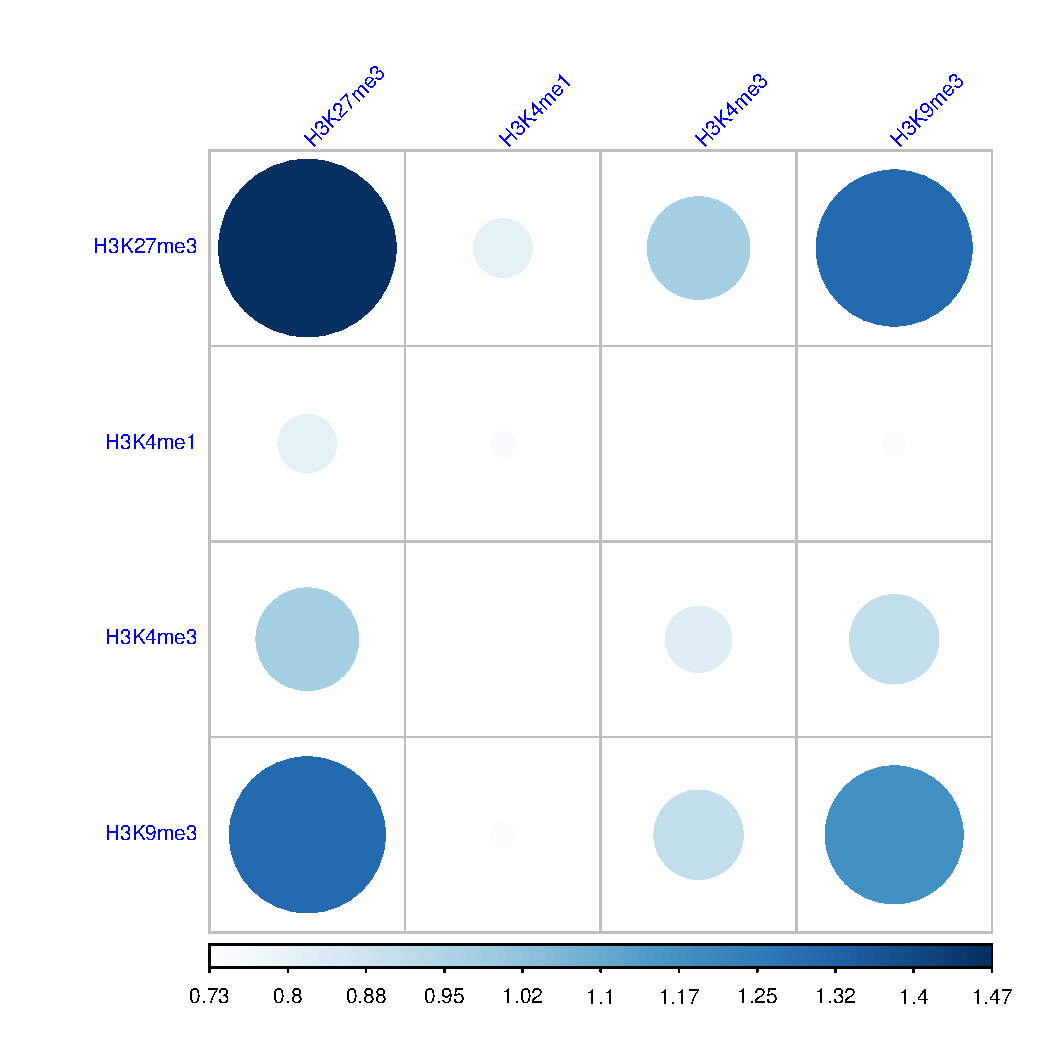
\includegraphics[width=\textwidth,height=0.5\textheight,keepaspectratio]{figure/annotations-stats_enrichment}
    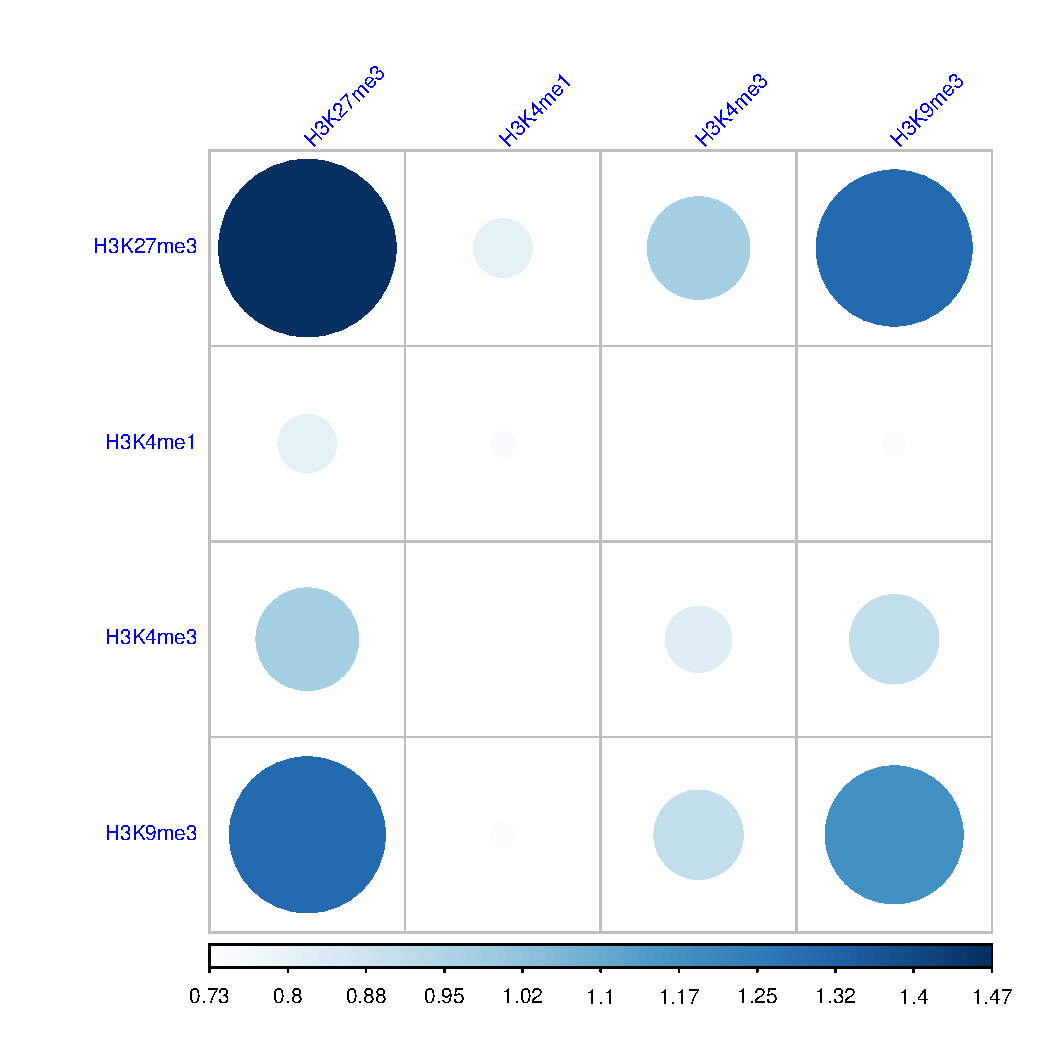
\includegraphics[width=\textwidth,height=\textheight,keepaspectratio]{figure/annotations-stats_enrichment}
    \caption{Annotation Stats enrichment sample output. See Section~\ref{HiC:annotations-stats}.} % results/annotations-stats.by_sample.standard/annotations.by_sample.standard/interactions.by_sample.standard/matrix-filtered.by_sample.res_10kb.maxd_5Mb.rotate45/filter.by_sample.standard/align.by_sample.bowtie2/CD34-HindIII-rep1/enrichment.pdf
    \label{fig:annotations-stats}
\end{figure}
% \newpage
\clearpage